\documentclass[11pt,a4paper]{article}
\usepackage{fontspec}\usepackage[margin=2.2cm]{geometry}\usepackage{graphicx,booktabs,float,tikz,hyperref,parskip,caption}
\usetikzlibrary{arrows.meta,positioning}\captionsetup{font=small}\hypersetup{colorlinks=true,linkcolor=black,urlcolor=blue}
\title{Shadow Squad: who replaces whom?\\[4pt]\large End-semester report, Player Replacement Scouting\\Analysis and Systems of Big Data, IIITDM Kancheepuram}\date{}
\begin{document}\sloppy\maketitle
\noindent This part follows the mid-semester report, which is included unchanged before it. Every number below is read from \texttt{outputs/metrics.json}, which the notebooks \texttt{endsem\_01} to \texttt{endsem\_06} write when they run.

\section{What changed since the mid-semester version, and why}
The mid-sem project asked which young players at smaller clubs will move up. Its main result was that no method clearly beat ranking the best young performers, and its cosine shortlist was worse than that baseline. Three things were limiting it, and the end-sem version changes all three.

\textbf{The question.} A club does not buy "a player who will move up". It buys a replacement for a specific starter who left. The end-sem system takes an elite club, a season and a departing starter, and returns a ranked list of candidates. The test is whether the player the club really signed is near the top of that list.

\textbf{The labels.} Mid-sem outcomes were inferred from the club a player's name appeared next to one or two seasons later. They are now taken from Transfermarkt transfer records. On the 1,953 feeder-seasons that have both labels, the two agree on "moved up" for 90.8\%. The old rule called 149 moves that have no matching permanent transfer; most are loan spells and loan returns, and 23 belong to players with no transfer record in the Transfermarkt dump. On the same rows the move-up rate falls from 26.6\% to 20.5\%. The transfer label also covers 2022-23 and 2023-24, which the old rule could not label.

\textbf{The data.} Transfermarkt (\texttt{davidcariboo/player-scores}) adds transfers, fees, market values, fine positions and a stable player id. FBref removed its advanced statistics in January 2026, so the seasons stay 2017-18 to 2023-24. A Kaggle scrape with 2024-25 exists (\texttt{emrey3lmaz}) but was not merged; Transfermarkt already supplies the 2024-25 minutes and transfers that the outcomes need.

The mid-sem notebook was re-run unchanged first. The minutes column it uses is named \texttt{avg\_mins\_per\_match} but holds season totals (maximum 3420), so no fix was needed. Its baseline on the refined labels: feeder base rate 26.7\%; best walk-forward model, logistic regression, 46 hits in 75 picks; best-composite baseline 31 in 75.

\section{Data lake and PySpark pipeline}
\begin{figure}[H]\centering\resizebox{\linewidth}{!}{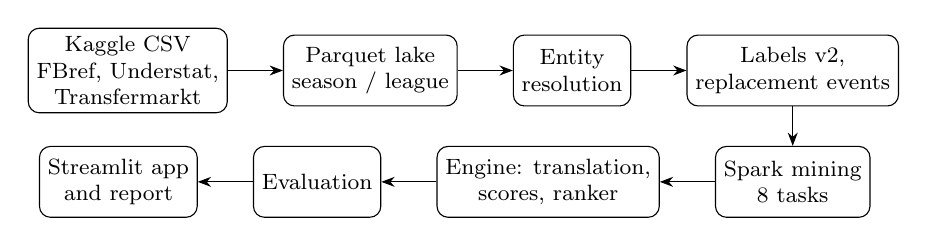
\begin{tikzpicture}[node distance=5mm and 7mm, b/.style={draw,rounded corners,align=center,font=\footnotesize,minimum height=9mm,inner sep=3pt}, >=Stealth]
\node[b](a){Kaggle CSV\\FBref, Understat,\\Transfermarkt};\node[b,right=of a](l){Parquet lake\\season / league};\node[b,right=of l](x){Entity\\resolution};\node[b,right=of x](e){Labels v2,\\replacement events};
\node[b,below=of e](mi){Spark mining\\8 tasks};\node[b,left=of mi](en){Engine: translation,\\scores, ranker};\node[b,left=of en](ev){Evaluation};\node[b,left=of ev](ap){Streamlit app\\and report};
\draw[->](a)--(l);\draw[->](l)--(x);\draw[->](x)--(e);\draw[->](e)--(mi);\draw[->](mi)--(en);\draw[->](en)--(ev);\draw[->](ev)--(ap);
\end{tikzpicture}}\caption{Pipeline. Every box after the first reads and writes Parquet under \texttt{lake/}.}\end{figure}
All sources are written as Parquet partitioned by season and league: \texttt{fbref} (10,355 player-seasons), \texttt{fbref\_raw} (18,243), \texttt{understat\_team} (684 club-seasons), \texttt{tm\_transfers} (168,248), \texttt{tm\_valuations} (615,190), \texttt{tm\_players} (50,149), plus two derived tables: league minutes per player, club and season, and league tables rebuilt from match results. The rebuilt tables agree with the mid-sem table on 99.1\% of club-seasons. Writing the lake takes 22 s in local mode. A query for one season and league reads one partition (the plan in notebook 01 shows the partition filter).

\textbf{Entity resolution.} FBref has no player id. Pass one learns the club alias map from the data: join on season, league, birth year and exact name key, then give each FBref club the Transfermarkt club most of its players belong to. All 145 clubs map one to one. Pass two blocks on (season, club) and compares accent-insensitive, token-sorted name keys with Spark \texttt{levenshtein} and a Jaro-Winkler pandas UDF, adds birth year and position group, and keeps mutual best pairs. It links 16,474 of 16,865 outfield player-club-seasons (97.7\%), and 99.1\% of those with 900 minutes or more; the worst league-season is 98.1\%. 33 of 2,751 feeder-seasons stay unmatched and are listed in \texttt{outputs/unmatched\_feeders.csv}.
\begin{figure}[H]\centering\includegraphics[width=0.7\linewidth]{/home/srioo/Desktop/Projects/root/BigP/bigdata/outputs/figs/p1_match_rate.png}\caption{Match rate per league and season for players with at least 900 minutes.}\end{figure}

\textbf{Replacement events.} An event is an elite club whose starter (1,350 minutes or more) plays under 450 league minutes for it the next season, and which signs a player of the same fine position in the summer between, who then plays at least 450 minutes. Loans are removed by walking each player's moves in date order (23,044 loan departures found). This gives 464 events from 371 signings. Only 23.2\% of those signings (86) were inside the candidate pool (age 26 or under, 900 minutes, non-elite club in the five leagues). 24.3\% came from clubs outside the five leagues, such as Benfica or Feyenoord, and the rest were older, at another elite club, or had played too little. The engine can only be right about the 95 events whose signing was in the pool, and all results below are restricted to them.
\begin{figure}[H]\centering\includegraphics[width=0.9\linewidth]{/home/srioo/Desktop/Projects/root/BigP/bigdata/outputs/figs/p2_labels_events.png}\caption{Left: mid-sem label against the transfer label. Right: share of real replacement signings that came from a five-league club and that were inside the candidate pool.}\end{figure}


\section{Post-mid-semester topics: one new algorithm per task, in PySpark}
None of these was used before the mid-sem. Each runs in Spark (local mode) with its plan shown once in notebook 03.

\begin{table}[H]\centering\footnotesize\begin{tabular}{p{2.6cm}p{4.0cm}p{6.6cm}r}\toprule
Task & Algorithm (Spark) & Result & Time (s)\\\midrule
Similarity search & Euclidean LSH, MinHash LSH & 95\% of true top-25 neighbours kept while comparing 88\% of pairs; both views together keep 95\% of real signings & 0.4\\
Sequential patterns & PrefixSpan & 477 frequent career sequences, 176 with lift $\geq$ 1.3; flagged players move up 27.5\% vs 25.0\% out of time & 1.0\\
Clustering & Bisecting k-means per fine position & 23 archetypes, mean silhouette 0.17; Cramer's V with moving up 0.20 & 56\\
Link analysis & GraphFrames PageRank; power-iteration clustering & pipeline rank alone AUC 0.573 (sales count 0.579); communities with modularity 0.32 & 22\\
Recommendation & ALS, implicit feedback & MRR 0.631 vs popularity 0.697: ALS loses & 13\\
Classification & LinearSVC, multilayer perceptron & LinearSVC AUC 0.687, MLP 0.558 (mid-sem best 0.681) & 147\\
Outlier detection & k-NN distance score (self-join) & hidden-gem flag: 15.0\% move up vs 22.2\% & 4.4\\
Stream mining & Structured Streaming, Count-Min Sketch & live team dominance reaches r = 0.9 with the season value after about 12 matches & 10\\\bottomrule
\end{tabular}\caption{The eight Spark mining tasks.}\end{table}

\textbf{Similarity search (LSH).} Random-projection LSH hashes vectors so that close ones tend to share a bucket, and only bucket-mates are compared. It generates the candidates for each event from style-neutral vectors; MinHash on top-quartile trait sets is the second view. The honest reading is that the pool is small (about 96 same-position players per event), so LSH saves little here: the chosen setting (4 hash tables, bucket length 2) still compares 88\% of pairs. It is in the pipeline because the same code scales to a pool of every league in the world.
\begin{figure}[H]\centering\includegraphics[width=0.55\linewidth]{/home/srioo/Desktop/Projects/root/BigP/bigdata/outputs/figs/p3_lsh_tradeoff.png}\caption{LSH: share of pairs compared against recall of the exact top-25 neighbours and of the real signings.}\end{figure}

\textbf{Sequential patterns (PrefixSpan).} A career is an ordered list of seasons, each an itemset of club tier, league, role and form band. PrefixSpan mines the frequent orders on feeder-seasons up to 2019. The strongest multi-season pattern is \{lg=SA\} $\rightarrow$ \{club=mid, form=mid\} (lift 2.34 in training, 1.06 later). Out of time the flagged group moves up at 1.10 times the base rate (Fisher p = 1.7e-07): a real but small signal, and the train and test lifts of individual patterns correlate only 0.26.
\begin{figure}[H]\centering\includegraphics[width=0.85\linewidth]{/home/srioo/Desktop/Projects/root/BigP/bigdata/outputs/figs/p3_prefixspan.png}\caption{Top career sequences by lift for moving up, in training and in later seasons.}\end{figure}

\textbf{Clustering (bisecting k-means).} Bisecting k-means splits the worst cluster in two repeatedly. It is run inside each of the seven Transfermarkt fine positions, which the mid-sem could not do with three coarse groups. It finds 23 archetypes; archetype and moving up are associated (chi-square p = 2.9e-14, Cramer's V 0.20). Creative archetypes are bought more often than defensive ones at every position.
\begin{figure}[H]\centering\includegraphics[width=0.95\linewidth]{/home/srioo/Desktop/Projects/root/BigP/bigdata/outputs/figs/p3_bisecting.png}\caption{Silhouette by k for each position, and the archetype centroids.}\end{figure}

\textbf{Link analysis (PageRank, PIC).} Each permanent transfer is an edge (61,230 in all). With edges pointing from buyer to seller, PageRank is high for clubs whose players are bought by important clubs. Academies and one-off amateur clubs had to be removed first, because the reversed graph rewards them. The top of the 2023 list is Salzburg, Indep. Medellín, Olympiacos, Benfica, Boca Juniors. For feeders, the club's pipeline rank alone gives AUC 0.573, which is no better than simply counting the club's past sales (0.579). Power-iteration clustering on 1,001 clubs gives transfer communities with modularity 0.32; the iteration count has to be chosen (here by modularity), because too many iterations collapse every club into one group.
\begin{figure}[H]\centering\includegraphics[width=0.95\linewidth]{/home/srioo/Desktop/Projects/root/BigP/bigdata/outputs/figs/p3_graph.png}\caption{Left: clubs with the highest talent-pipeline PageRank. Right: transfer communities by league.}\end{figure}

\textbf{Recommendation (ALS).} ALS factorises the club by archetype matrix of past signings. This did not work. On 1,119 later signings, ALS ranks the bought archetype worse than league-wide popularity (MRR 0.631 against 0.697; difference 95\% interval [-0.085, -0.047]). The training matrix has only 364 signings across 132 clubs, too few to learn a club's taste. The score is kept in the engine so the ablation can measure it.
\begin{figure}[H]\centering\includegraphics[width=0.45\linewidth]{/home/srioo/Desktop/Projects/root/BigP/bigdata/outputs/figs/p3_als.png}\caption{Mean reciprocal rank of the archetype a club actually bought.}\end{figure}

\textbf{Classification (LinearSVC, MLP).} Same question and same walk-forward split as the mid-sem classifiers. LinearSVC reaches AUC 0.687 with 41 hits in 75 picks, level with the mid-sem logistic regression (0.681, 46 hits). The perceptron overfits the 700 to 1,900 training rows and is clearly worse (AUC 0.558). On the transfer label over five test seasons LinearSVC gets AUC 0.680 and 62 hits in 125.
\begin{figure}[H]\centering\includegraphics[width=0.62\linewidth]{/home/srioo/Desktop/Projects/root/BigP/bigdata/outputs/figs/p3_classification.png}\caption{New Spark classifiers next to the mid-sem leaderboard (same label, same test seasons).}\end{figure}

\textbf{Outlier detection (k-NN distance).} The score is the mean distance to the ten nearest neighbours inside the archetype. Unusual players are bought slightly more often (Spearman -0.088, p = 0.000). The hidden-gem flag (top decile of the score and above-median composite index) marks 100 feeders who moved up at 15.0\% against 22.2\% for the rest (Fisher p = 9.7e-01).
\begin{figure}[H]\centering\includegraphics[width=0.5\linewidth]{/home/srioo/Desktop/Projects/root/BigP/bigdata/outputs/figs/p3_outlier.png}\caption{Move-up rate by decile of the k-NN outlier score.}\end{figure}

\textbf{Stream mining.} The 2023-24 Understat matches are replayed one week per micro-batch (39 batches). A stateful aggregation keeps each team's running dominance; after five weeks it correlates 0.80 with the end-of-season value and passes 0.9 at about 12 matches per team. A Count-Min Sketch counts deep completions per team in fixed memory: at width 200 the mean relative error is 0.0\%, and at width 20 it over-counts by 2.5 times the true count, which shows what the width buys.
\begin{figure}[H]\centering\includegraphics[width=0.5\linewidth]{/home/srioo/Desktop/Projects/root/BigP/bigdata/outputs/figs/p3_stream.png}\caption{Streaming team dominance against the end-of-season value.}\end{figure}


\section{Techniques beyond the course}
\textbf{Survival analysis.} Feeder-seasons become person-period rows (2,562 rows, 314 events), which lets the last two seasons be used (697 rows). The discrete-time hazard is a Spark logistic regression refitted each season on past rows only; its walk-forward AUC is 0.688 and its predicted and observed rates differ by 2.2\% on average across deciles. On 819 later entrants its concordance index is 0.675; a Cox proportional-hazards model (\texttt{lifelines}) fitted as a check gets 0.656.

\textbf{Learning to rank.} LightGBM \texttt{LGBMRanker} (LambdaMART) with one query per replacement event, against a pointwise Spark \texttt{GBTClassifier}. Section 6 has the results.

\textbf{Conformal prediction.} Split-conformal turns a score into a list with a stated coverage. For movers: to catch 90\% of next season's real movers the hazard list must hold 84\% of all feeders, and it then caught 94.5\% on later seasons; a 50\% promise needs 26\% of feeders and caught 43.8\%. For replacement events, calibrated on 26 events and checked on 38: a list that contains the real signing 90\% of the time needs 70\% of the pool (about 70 players) and covered 86.8\%; a 50\% promise needs about 32 players and covered 57.9\%. The guarantees hold approximately, and they show that a short list cannot promise much.
\begin{figure}[H]\centering\includegraphics[width=1.0\linewidth]{/home/srioo/Desktop/Projects/root/BigP/bigdata/outputs/figs/p5_calibration_coverage.png}\caption{Hazard calibration, conformal coverage on later seasons, and the list size a guarantee costs.}\end{figure}

\textbf{SHAP} (TreeExplainer on the ranker) explains each candidate's rank, and \textbf{dynamic time warping} is compared with the simple trajectory similarity: the two correlate 0.43 and put the real signing in the top 10 equally often (17\% and 17\%), so DTW adds nothing here. Only 14\% of pairs could be age-aligned, because the starter's seasons at the candidate's age are usually before 2017.

\section{Style translation and its check on real movers}
The mid-sem removed team style from a player's numbers. Translation runs it the other way, into the buying club:
\[\mathrm{stat\ in\ }C = \mathrm{stat}_{\mathrm{neutral}} \times \exp\Big(\sum_{\mathrm{supported\ terms}} \beta_{\mathrm{pos,metric,term}}\, x_{\mathrm{term}}(C,t)\Big) \times \mathrm{league\ factor}(C)\]
using the mid-sem elasticities and league offsets unchanged. The check uses 1,110 players who changed club between consecutive seasons (460 across leagues). Their per-90 numbers at the new club are predicted from (a) last season's raw numbers, (b) style-neutral numbers, and (c) neutral numbers translated into the new club, using the club's style from the season before the move.

Mean absolute error, in standard deviations of each metric: (a) 0.495, (b) 0.486, (c) 0.489. Translation beats raw numbers by a small amount (difference [-0.010, -0.003], 95\% bootstrap) and in 37 of 48 position-by-metric cells. It does not beat the plain style-neutral numbers (difference [-0.001, +0.006]). Most of the gain is from removing the old club's style; adding the new club's style contributes nothing measurable, even with the new club's true style that season (0.484). So translation is kept as a display feature (the radar) and as one ranking score, with the gain over raw numbers stated at about 1.2\% of the error.
\begin{figure}[H]\centering\includegraphics[width=0.85\linewidth]{/home/srioo/Desktop/Projects/root/BigP/bigdata/outputs/figs/p4_translation.png}\caption{Error in predicting a mover's next-season per-90s, by metric.}\end{figure}


\section{Results}
For each event the engine scores every same-position pool player on translated similarity, trajectory similarity, the selling club's pipeline PageRank, the buying club's ALS taste, the survival hazard, and market value (level, and gap to the departing starter), with age and composite index. A LambdaMART ranker combines them. It is trained walk-forward: events of season $Y$ are ranked by a model that saw only events up to $Y-1$. The test set is 64 events from 2020-21 to 2023-24, with about 101 candidates each.

\begin{table}[H]\centering\footnotesize\resizebox{\linewidth}{!}{\begin{tabular}{lrrrrrr}\toprule
Method & Median rank & R@5 & R@10 [95\% CI] & R@25 & R@50 & p vs best young\\\midrule
Random order of the pool & 46.0 & 6\% & 12\% [5, 20] & 28\% & 55\% &  \\
Highest market value & 19.2 & 14\% & 27\% [16, 38] & 62\% & 78\% & 0.27 \\
Raw cosine similarity to the starter & 35.0 & 12\% & 25\% [14, 36] & 36\% & 62\% & 0.36 \\
Best young performer (composite index) & 29.5 & 5\% & 17\% [8, 27] & 41\% & 66\% &  \\
\midrule
Single score: hazard & 22.5 & 17\% & 28\% [17, 39] & 56\% & 78\% & 0.06 \\
Single score: translated similarity & 36.5 & 14\% & 22\% [12, 33] & 31\% & 62\% & 0.63 \\
\midrule
Shadow Squad fusion with Spark GBT (pointwise) & 34.5 & 2\% & 14\% [6, 23] & 38\% & 70\% & 0.81 \\
\textbf{Shadow Squad (LambdaMART, all scores)} & 26.0 & 12\% & 31\% [20, 42] & 47\% & 73\% & 0.08 \\
Ablation: no translation & 28.5 & 6\% & 19\% [9, 28] & 47\% & 73\% & 1.00 \\
Ablation: no trajectory & 25.5 & 11\% & 25\% [14, 36] & 50\% & 75\% & 0.37 \\
Ablation: no PageRank & 26.5 & 17\% & 25\% [16, 36] & 48\% & 73\% & 0.36 \\
Ablation: no ALS taste & 26.0 & 14\% & 23\% [14, 34] & 48\% & 75\% & 0.48 \\
\bottomrule\end{tabular}}\caption{Replacement recall@K and median rank of the real signing on 64 unseen in-pool events. Intervals are bootstrap over events; the last column is a paired permutation test on recall@10 against the best-young-performer baseline.}\end{table}

\textbf{What worked.} Shadow Squad puts the real signing in the top 10 for 31\% of events. A random order gets 12\%, the mid-sem method (raw cosine similarity) 25\%, and the mid-sem result to beat (best young performer) 17\%. That is the highest recall@10 in the table.

\textbf{What did not.} With 64 events the difference from the best-young-performer baseline is not statistically significant (p = 0.08; difference in recall@10 [+0.00, +0.28]). Two single scores do about as well as the full engine: the highest market value has a better median rank (19.2 against 26.0) and better recall@25 (62\% against 47\%), and the hazard alone reaches 28\% at 10 and 56\% at 25. Elite clubs mostly sign the players everyone already values. The pointwise Spark GBT is worse than LambdaMART (14\% at 10).

\textbf{Ablation.} Removing one score at a time changes recall@10 from 31\% to 19\% without translation, 25\% without trajectory, 25\% without PageRank and 23\% without ALS taste. Every interval overlaps the full model's, so no single score can be said to matter on this many events. Translation shows the largest drop.
\begin{figure}[H]\centering\includegraphics[width=1.0\linewidth]{/home/srioo/Desktop/Projects/root/BigP/bigdata/outputs/figs/p5_recall_ablation.png}\caption{Left: recall@K with 95\% bootstrap bands. Right: recall@10 with one score removed at a time.}\end{figure}

\begin{figure}[H]\centering\includegraphics[width=0.6\linewidth]{/home/srioo/Desktop/Projects/root/BigP/bigdata/outputs/figs/p6_shap_global.png}\caption{Mean absolute SHAP value of each score on unseen events.}\end{figure}


\section{Model predictions, with an explanation for each}
The screenshots are from the Streamlit app (\texttt{app/shadow\_squad.py}), which reads the Parquet lake: choose a league, an elite club, a season and a departing starter. It shows the ranked list, what the club really did, the radar (starter's actual numbers, candidate raw, candidate translated into the club), the SHAP waterfall for the chosen candidate, and market values. The cases were picked by rule: the three unseen events with the best rank for the real signing, and the unseen event where a real signing was ranked worst.

\section{Case studies}
\subsection*{Three hits}
\paragraph{Dortmund 2023-24: Niclas Füllkrug (ST) replaced by Maximilian Beier from Hoffenheim (fee EUR 28.5m).} The engine ranked him 2 of 76 pool players at that position. His strongest scores were move-up hazard (higher than 91\% of the pool), market value (higher than 88\% of the pool), club pipeline rank (higher than 86\% of the pool). The first name on the list was Elye Wahi (Lens).
\begin{figure}[H]\centering\includegraphics[width=0.92\linewidth]{/home/srioo/Desktop/Projects/root/BigP/bigdata/outputs/screens/hit_Dortmund_2023_Beier.png}\caption{Dashboard for this event: ranked list, translated radar and SHAP waterfall for Maximilian Beier.}\end{figure}
\paragraph{Paris S-G 2022-23: Neymar (AM) replaced by Kang-in Lee from RCD Mallorca (fee EUR 22.0m).} The engine ranked him 2 of 42 pool players at that position. His strongest scores were move-up hazard (higher than 95\% of the pool), translated similarity (higher than 93\% of the pool), trajectory similarity (higher than 81\% of the pool). The first name on the list was Gabriel Veiga (Celta Vigo).
\begin{figure}[H]\centering\includegraphics[width=0.92\linewidth]{/home/srioo/Desktop/Projects/root/BigP/bigdata/outputs/screens/hit_ParisS-G_2022_Lee.png}\caption{Dashboard for this event: ranked list, translated radar and SHAP waterfall for Kang-in Lee.}\end{figure}
\paragraph{Paris S-G 2021-22: Georginio Wijnaldum (CM) replaced by Carlos Soler from Valencia (fee EUR 18.0m).} The engine ranked him 2 of 104 pool players at that position. His strongest scores were move-up hazard (higher than 98\% of the pool), market value (higher than 97\% of the pool), composite index (higher than 75\% of the pool). The first name on the list was Pablo Fornals (West Ham).
\begin{figure}[H]\centering\includegraphics[width=0.92\linewidth]{/home/srioo/Desktop/Projects/root/BigP/bigdata/outputs/screens/hit_ParisS-G_2021_Soler.png}\caption{Dashboard for this event: ranked list, translated radar and SHAP waterfall for Carlos Soler.}\end{figure}

\subsection*{One miss}
\paragraph{Marseille 2022-23: Sead Kolašinac (CB) replaced by Bamo Meïté from FC Lorient (fee EUR 10.5m).} The engine ranked him 131 of 133, close to last. His weakest scores were market value (higher than 2\% of the pool), age (higher than 2\% of the pool), composite index (higher than 8\% of the pool). His market value was EUR 1.5m against EUR 5.0m for the starter he replaced. The ranker has learned that elite clubs mostly buy established, highly valued players, so a cheap squad signing with a thin record is exactly the kind of move it cannot see coming.
\begin{figure}[H]\centering\includegraphics[width=0.92\linewidth]{/home/srioo/Desktop/Projects/root/BigP/bigdata/outputs/screens/miss_Marseille_2022_Meïté.png}\caption{Dashboard for this event: ranked list, translated radar and SHAP waterfall for Bamo Meïté.}\end{figure}


\section{Limitations and conclusion}
\begin{itemize}
\item Coverage. 77\% of real replacement signings were outside the candidate pool, most of them from leagues the data does not cover. The engine is evaluated only on the rest.
\item Sample size. 95 in-pool events in seven seasons, 64 of them unseen. The intervals are wide and the method order in the results table is not reliable.
\item Transfer records. 9.1\% of feeder-seasons belong to players with no record in the Transfermarkt dump and are labelled "no move". Loans are inferred from move patterns, not from a loan flag.
\item The style elasticities, league offsets, archetypes and outlier scores are fitted on all seasons without outcome labels, as in the mid-sem. The ranker, hazard, PageRank and ALS scores use only past data.
\item Local Spark. Everything runs in local mode on one machine; the data is far smaller than what Spark is for.
\end{itemize}
Reframing the task as "who replaces whom" gives a test that the mid-sem lacked: a real decision by a real club. On that test the engine has the best top-10 recall of the methods tried and nearly doubles the mid-sem baseline, but the margin is not significant on 64 events, and market value alone is as good or better deeper in the list. Style translation improves on raw numbers by about 1.2\% and no more than style-neutral numbers do. The parts that held up are the transfer-based labels, the entity resolution, the survival hazard, and a dashboard that shows why each candidate is ranked where he is.
\end{document}
